% ============================================================================
\section{Simulating seizures}
\label{sec:sim}

The question ``can we simulate epilepsy?'' was answered with three models of increasing realism, all run with \code{uv}. The third, \code{ionic.py}, was requested to be ``as close to real life as possible'', with potassium and chloride build-up; wherever something looked wrong, the literature was consulted and the model changed.

\begin{table}[H]
\centering\small
\caption{The three models.}
\begin{tabularx}{\linewidth}{@{}l L L L@{}}
\toprule
& Model 1: spiking network & Model 2: Epileptor & Model 3: ionic model \\
\midrule
Type & 1,000 Izhikevich neurons & 6 ODEs, phenomenological & 100 Hodgkin--Huxley neurons with ion concentrations \\
Seizure cause & GABA strength cut by hand & Slow variable $z$ crosses a threshold & Emerges from \Kp/\Clm/\Nap/adenosine dynamics and pathology \\
Termination & Inhibition restored by hand & $z$ dynamics & Pump, \Nap-activated \Kp{} current, adenosine \\
Variables & Spikes, LFP proxy & Abstract & \Ko, \Nai, \Cli, \EGABA, $E_K$, pump flux, adenosine, CBF, HbO, HbR \\
Validated against & Qualitative & Jirsa 2014 behaviour; TVB (\S\ref{sec:tvb}) & Cressman 2009 Fig.~1 (quantitative) \\
Runtime & $\approx$5\,s & $\approx$2\,s & 7\,s (validate) to $\approx$6\,min \\
\bottomrule
\end{tabularx}
\end{table}

\subsection{Model 1: spiking network with inhibition failure}

800 regular-spiking excitatory and 200 fast-spiking inhibitory Izhikevich neurons,
\begin{equation}
\dot v = 0.04v^2 + 5v + 140 - u + I,\qquad \dot u = a(bv-u),\qquad v\ge 30\,\mathrm{mV}\Rightarrow v\leftarrow c,\ u\leftarrow u+d .
\end{equation}
GABA weights were scaled to 0.35 between 1.5 and 2.8\,s. A synchrony index (variance of the population rate divided by the mean single-cell variance) rose from \textbf{0.02} (baseline) to \textbf{0.98} (inhibition weakened) and returned to 0.02, reproducing hypersynchronous population bursts (Figure~\ref{fig:net}).

\begin{figure}[H]
\centering
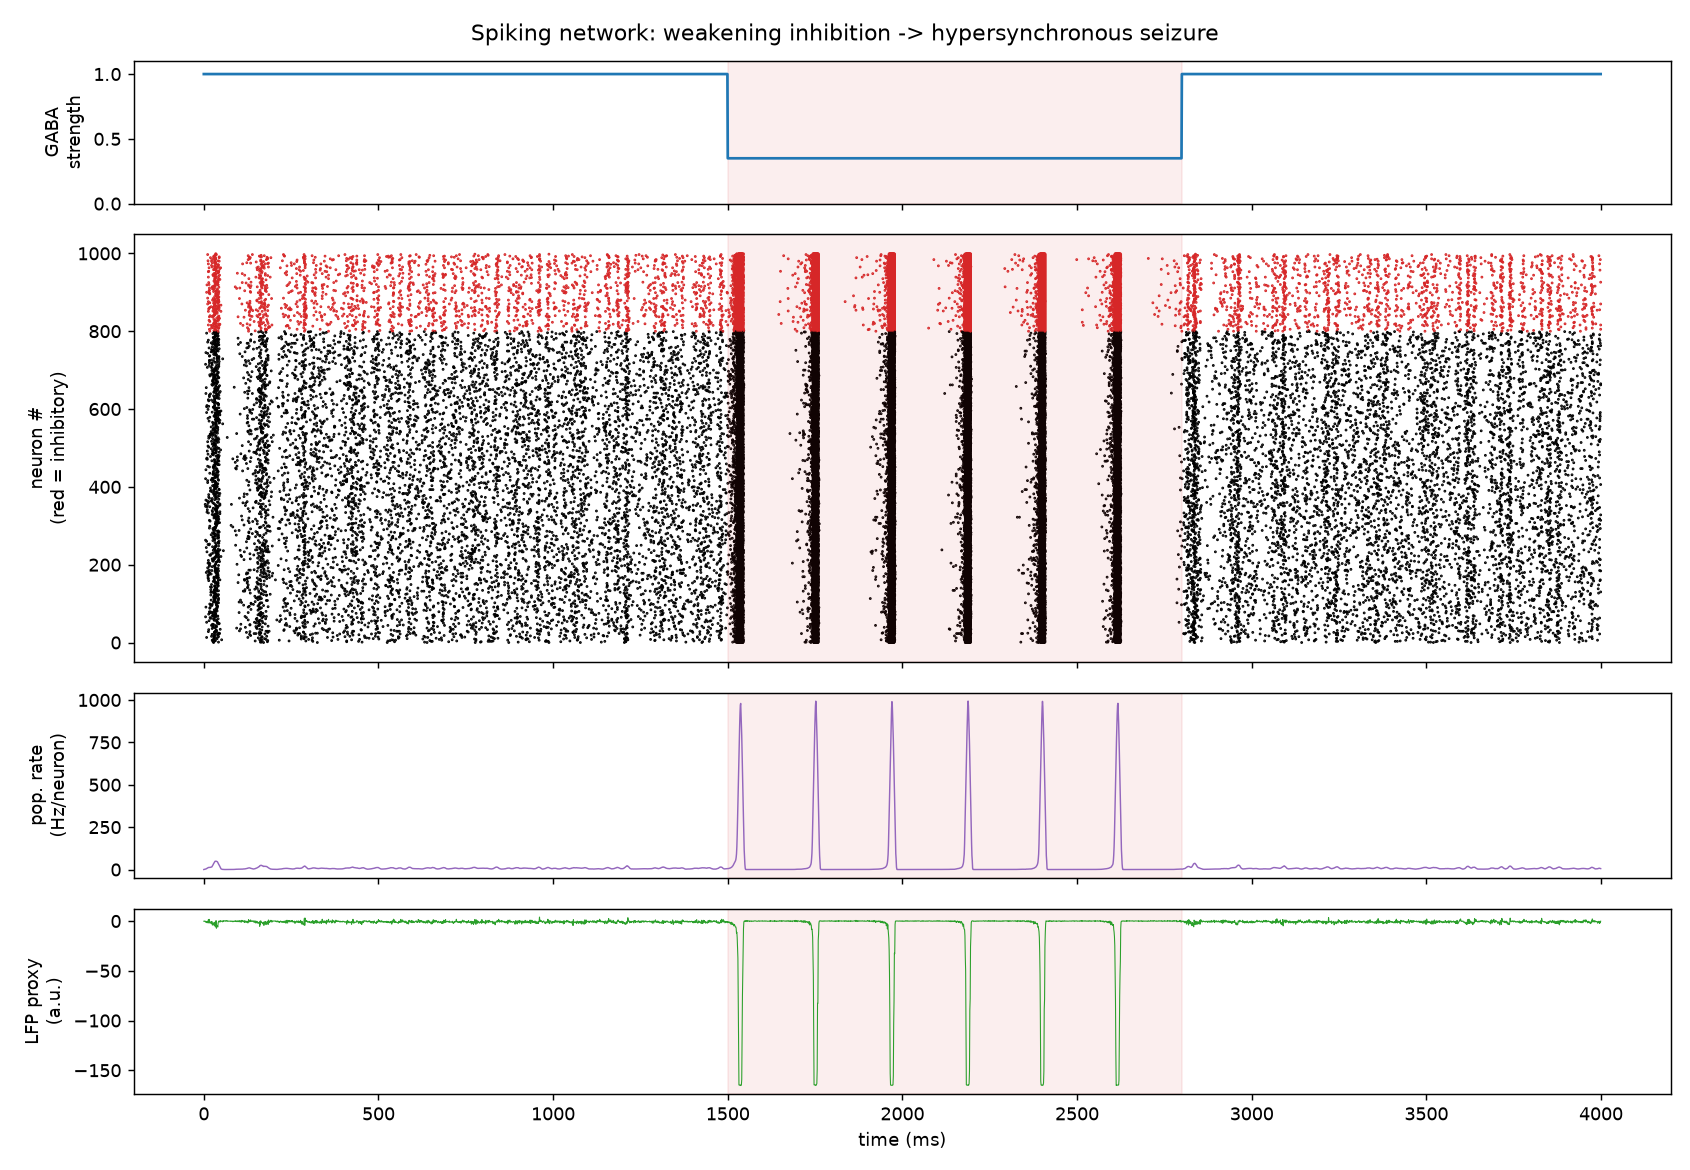
\includegraphics[width=0.78\linewidth]{epilepsy_sim/output/network_seizure.png}
\caption{Model 1: weakening inhibition turns asynchronous firing into lock-step population bursts.}
\label{fig:net}
\end{figure}

\subsection{Model 2: the Epileptor}

The Epileptor (Jirsa et al.\ 2014), the engine of The Virtual Brain, has two fast oscillators, a slow permittivity variable $z$ and a coupling term $g$:
\begin{align}
\dot x_1 &= y_1 - f_1(x_1,x_2) - z + I_1, & \dot y_1 &= y_0 - 5x_1^2 - y_1,\\
\dot z &= \tfrac{1}{\tau_0}\big(4(x_1-x_0) - z\big), & \dot x_2 &= -y_2 + x_2 - x_2^3 + I_2 + 2g - 0.3(z-3.5),\\
\dot y_2 &= \tfrac{1}{\tau_2}\big(-y_2 + f_2(x_2)\big), & \dot g &= -0.01\,(g - 0.1x_1).
\end{align}
With $x_0=-1.6$ the model produced 3 seizures in 6,000 time units (51.6\% of time ictal); with $x_0=-2.2$ (``healthy'') it produced none.

\begin{figure}[H]
\centering
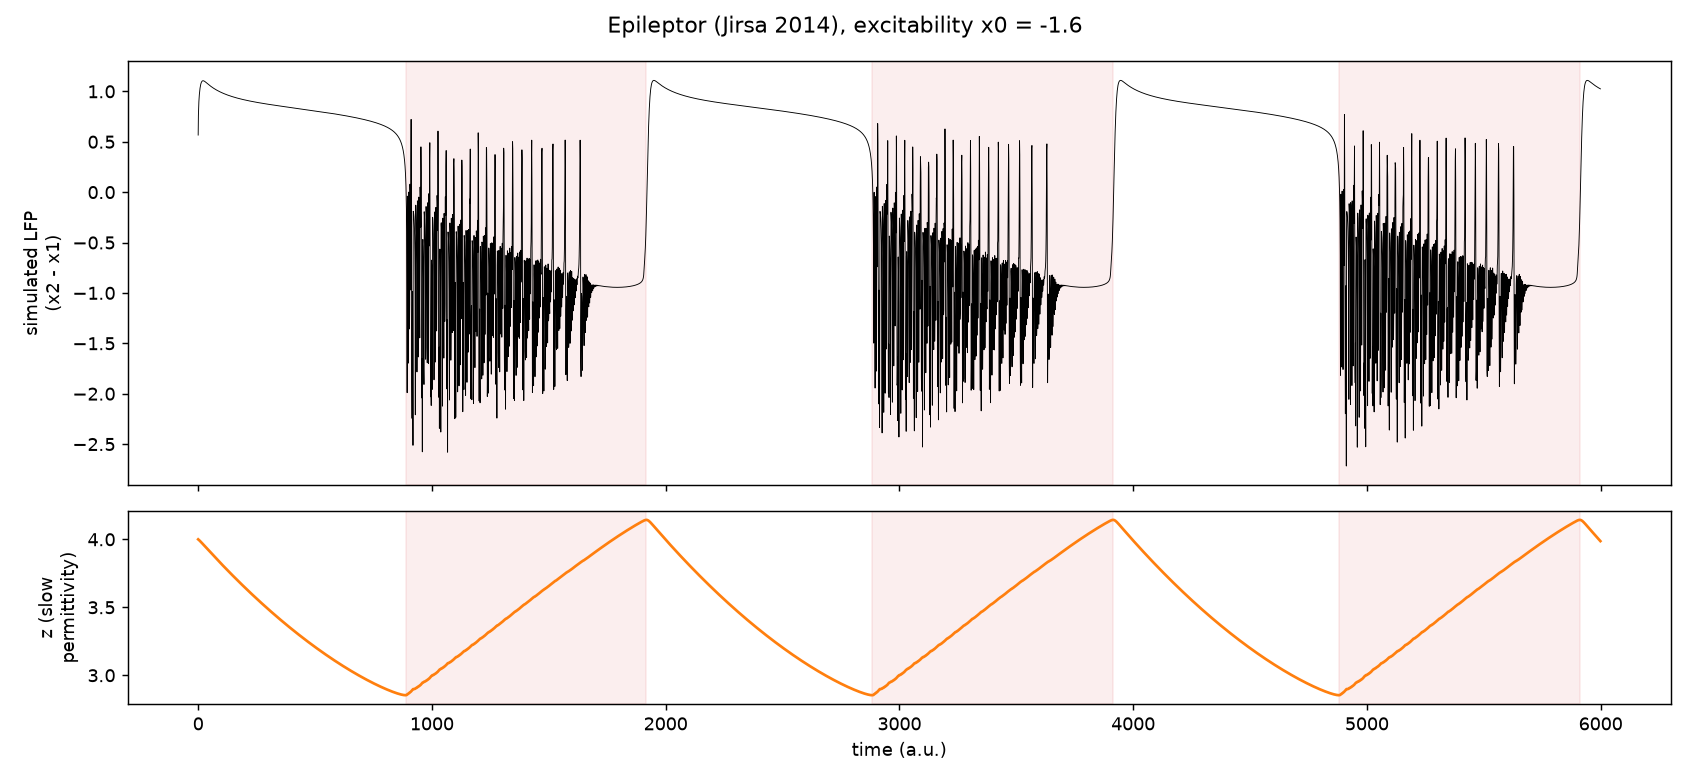
\includegraphics[width=0.78\linewidth]{epilepsy_sim/output/epileptor_seizures.png}
\caption{Model 2: Epileptor seizures driven by the slow variable $z$.}
\end{figure}

\subsection{Model 3: the ionic seizure model}

\subsubsection{Architecture and feedback loops}

A seizure is modelled as a contest between fast positive and slow negative feedback: \Kp{} accumulation depolarises neurons (+, 0.1--5\,s); \Clm{} loading makes GABA depolarising (+, 1--30\,s); KCC2 extrudes \Kp{} together with \Clm{} (+, seconds); \Nap{} accumulation drives an electrogenic pump current and a \Nap-activated \Kp{} current (Slack) ($-$); pump ATP use produces adenosine that opens GIRK channels and reduces release ($-$, 5--60\,s); glia, diffusion and vasculature clear \Kp{} ($-$).

The network has 100 neurons on a ring (every fifth inhibitory: 80 E, 20 I), local random wiring within $\pm$10 cells ($p=0.6$ from E, $0.8$ from I), a private extracellular micro-compartment per cell coupled by lateral \Kp{} diffusion, and Poisson background excitation. State variables per neuron are $V$, gates $n,h$, $[\mathrm{Ca}]_i$, \Ko, \Nai, \Cli, $g_e$, $g_i$, vesicle resources $x$ (optional depression) and adenosine $A$; $[\mathrm{K}]_i = 158-[\mathrm{Na}]_i$ and $[\mathrm{Na}]_o = 144-\beta([\mathrm{Na}]_i-18)$.

\subsubsection{Equations}

Membrane (positive-outward convention):
\begin{equation}
C\frac{dV}{dt} = -\big(I_{Na} + I_K + I_{Cl} + I_{AMPA} + I_{GABA} + s_p I_{pump}\big),
\end{equation}
with intrinsic currents (Cressman 2009)
\begin{align}
I_{Na} &= g_{Na} m_\infty^3 h (V-E_{Na}) + g_{NaL}(V-E_{Na}),\\
I_K &= \Big(g_K n^4 + g_{AHP}\tfrac{[\mathrm{Ca}]_i}{1+[\mathrm{Ca}]_i} + g_{KNa}w_\infty([\mathrm{Na}]_i) + g_{GIRK}(A)\Big)(V-E_K) + g_{KL}(V-E_K),\\
I_{Cl} &= g_{ClL}(V-E_{Cl}),
\end{align}
classical Hodgkin--Huxley rates with $m$ at steady state and $\phi=3$. Reversal potentials use $RT/F=26.64$\,mV (Cressman's value, 36\,\textdegree C):
\begin{equation}
E_K = 26.64\ln\frac{[\mathrm{K}]_o}{[\mathrm{K}]_i},\quad
E_{Cl} = 26.64\ln\frac{[\mathrm{Cl}]_i}{[\mathrm{Cl}]_o},\quad
E_{GABA} = 0.8E_{Cl} + 0.2E_{HCO_3},\quad E_{HCO_3}\approx-12.9\ \mathrm{mV}.
\end{equation}
Synapses are exponential conductances ($\tau_{AMPA}=5$\,ms, $\tau_{GABA}=8$\,ms) split by ion so that they feed the concentration equations:
\begin{equation}
I_{AMPA} = 0.64g_e(V-E_{Na}) + 0.36g_e(V-E_K),\qquad I_{GABA} = 0.8g_i(V-E_{Cl}) + 0.2g_i(V-E_{HCO_3}).
\end{equation}
Pump, glia, diffusion and KCC2 (fluxes in mM/s; corrected ModelDB version):
\begin{align}
I_{pump} &= \frac{\rho}{1+e^{(25-[\mathrm{Na}]_i)/3}}\cdot\frac{1}{1+e^{5.5-[\mathrm{K}]_o}},\quad
I_{glia} = \frac{s_g G_{glia}}{1+e^{(18-[\mathrm{K}]_o)/2.5}},\quad
I_{diff} = s_c\varepsilon([\mathrm{K}]_o - K_{bath}),\\
J_{KCC2} &= s_k U_{KCC2}\ln\frac{[\mathrm{K}]_i[\mathrm{Cl}]_i}{[\mathrm{K}]_o[\mathrm{Cl}]_o}.
\end{align}
Concentrations ($\gamma=0.0445$ current-to-concentration, $\beta=7$ volume ratio, $\div1000$ for ms$\to$s):
\begin{align}
\frac{d[\mathrm{K}]_o}{dt} &= \tfrac{1}{1000}\big(\gamma\beta(I_K+I_{AMPA,K}) - 2\beta I_{pump} - I_{glia} - I_{diff} + \beta J_{KCC2}\big) + D_{lat}\nabla^2[\mathrm{K}]_o,\\
\frac{d[\mathrm{Na}]_i}{dt} &= \tfrac{1}{1000}\big(-\gamma(I_{Na}+I_{AMPA,Na}) - 3I_{pump}\big),\qquad
\frac{d[\mathrm{Cl}]_i}{dt} = \tfrac{1}{1000}\big(\gamma(I_{Cl}+I_{GABA,Cl}) - J_{KCC2}\big).
\end{align}
The electrogenic pump current is $I^{(\mu A/cm^2)}_{pump} = s_p I_{pump}/\gamma$. The Slack current uses the Compte et al.\ (2003) curve with its EC50 shifted from 38.7 to 68.6\,mM to match this model's resting \Nai: $w_\infty = 0.37/(1+(68.6/[\mathrm{Na}]_i)^{3.5})$. Adenosine is produced in proportion to pump ATP use above rest and cleared with $\tau_A=20$\,s:
\begin{equation}
\frac{dA}{dt} = \alpha_A\max(I_{pump}-0.25,0) - \frac{A}{\tau_A},\qquad g_{GIRK} = g_{ado}\frac{A}{1+A},\qquad \text{release}\times\frac{1}{1+A}.
\end{equation}
Neurovascular coupling uses the Balloon--Windkessel model (Friston et al.\ 2000) driven by $u = k\ln(\mathrm{rate}/\mathrm{baseline})$ clipped to $[0.3\times,30\times]$:
\begin{equation}
\dot s = u - \kappa s - \gamma_f(f-1),\quad \dot f = s,\quad \tau_0\dot v = f - v^{1/\alpha},\quad
\tau_0\dot q = \frac{f(1-(1-E_0)^{1/f})}{E_0} - v^{1/\alpha}\frac{q}{v},
\end{equation}
with CBF $=f$, HbT $\propto v$, HbR $\propto q$ and HbO $=(\mathrm{HbT}-0.4\,\mathrm{HbR})/0.6$.

\subsubsection{Parameters}

\begin{table}[H]
\centering\small
\caption{Main parameters of the ionic model and their sources.}
\begin{tabularx}{\linewidth}{@{}l l L@{}}
\toprule
Parameter & Value & Source / rationale \\
\midrule
$g_{Na}, g_K, g_{AHP}$ & 100, 40, 0.01 mS/cm\textsuperscript{2} & Cressman 2009 Table 1 \\
$g_{NaL}, g_{KL}, g_{ClL}$ & 0.0175, 0.05, 0.05 mS/cm\textsuperscript{2} & Cressman 2009 \\
$\gamma$, $\beta$ & 0.0445, 7 & ModelDB code (corrected by the 2011 erratum) \\
$\rho$, $G_{glia}$ & 1.25, 66.7 mM/s & Cressman 2009 \\
$\varepsilon$, $K_{bath}$ & 1.33 s\textsuperscript{$-1$}, 4 mM & Cressman code; plasma \Kp \\
$D_{lat}$ & 0.625 s\textsuperscript{$-1$} & $D=2.5\times10^{-6}$ cm\textsuperscript{2}/s, $\Delta x=20$ \textmu m \\
$[\mathrm{Cl}]_o$, $[\mathrm{HCO_3}]_{i/o}$ & 130, 16/26 mM & Standard physiology \\
$U_{KCC2}$ & 0.4 mM/s & Gives resting \Cli{} $\approx$5--6 mM, \EGABA{} $\approx-70$ mV \\
$g_{KNa}$ & 1.33 mS/cm\textsuperscript{2}, EC50 68.6 mM & Compte 2003, shifted \\
$g_{ado}, \alpha_A, \tau_A$ & 0.3 mS/cm\textsuperscript{2}, 0.5, 20 s & During \& Spencer 1992; Boison \\
Recurrent $g_E/g_I$ & 1.3 / 2.6 mS/cm\textsuperscript{2} & Balanced E/I, calibrated \\
Background & 60 Hz $\times$ 0.07 mS/cm\textsuperscript{2} & 4--6 Hz asynchronous baseline \\
Pump-current scale $s_p$ & 1.0 & See calibration log \\
Neurovascular gain $k$ & 0.12 & CBF rise of $\approx$+40--100\% \\
\bottomrule
\end{tabularx}
\end{table}

\subsubsection{Healthy vs epileptic tissue and numerics}

Both tissues share neurons and wiring; only the pathology, modelled on hippocampal sclerosis, differs: KCC2 $\times$0.3 (downregulated in human epileptic tissue), glial \Kp{} buffering $\times$0.3 (Kir4.1 loss) and vascular \Kp{} clearance $\times$0.35 (gliosis). Each run first settles for a 60\,s warm-up; at $t=10$--12\,s both receive the same 2\,s trigger (+400\,Hz excitatory input). Voltage and gates use exponential Euler, $V_{t+dt} = V_\infty + (V_t - V_\infty)e^{-dt\,g_{tot}}$, which stays stable when conductances become large (forward Euler produced NaN); $dt=0.02$\,ms; concentrations use forward Euler; the loop is numba-compiled (100 neurons $\times$ 360\,s in $\approx$6\,min).

\subsubsection{Validation}

With all additions switched off (fixed \Clm, no pump current, no $I_{KNa}$, no adenosine), a single neuron in 8\,mM bath \Kp{} reproduces Cressman et al.\ (2009) Fig.~1:

\begin{table}[H]
\centering\small
\caption{Validation against Cressman et al.\ 2009, Fig.~1.}
\begin{tabular}{@{}lll@{}}
\toprule
Quantity & Cressman 2009 & This implementation \\
\midrule
Seizure-like events & Periodic, every $\approx$30 s & Every $\approx$29.5 s \\
\Ko{} range & $\approx$6.7$\to$10.2 mM & 6.7$\to$10.7 mM \\
\Nai{} range & $\approx$16.3$\to$19 mM & 15.5$\to$19.1 mM \\
\bottomrule
\end{tabular}
\end{table}

\begin{figure}[H]
\centering
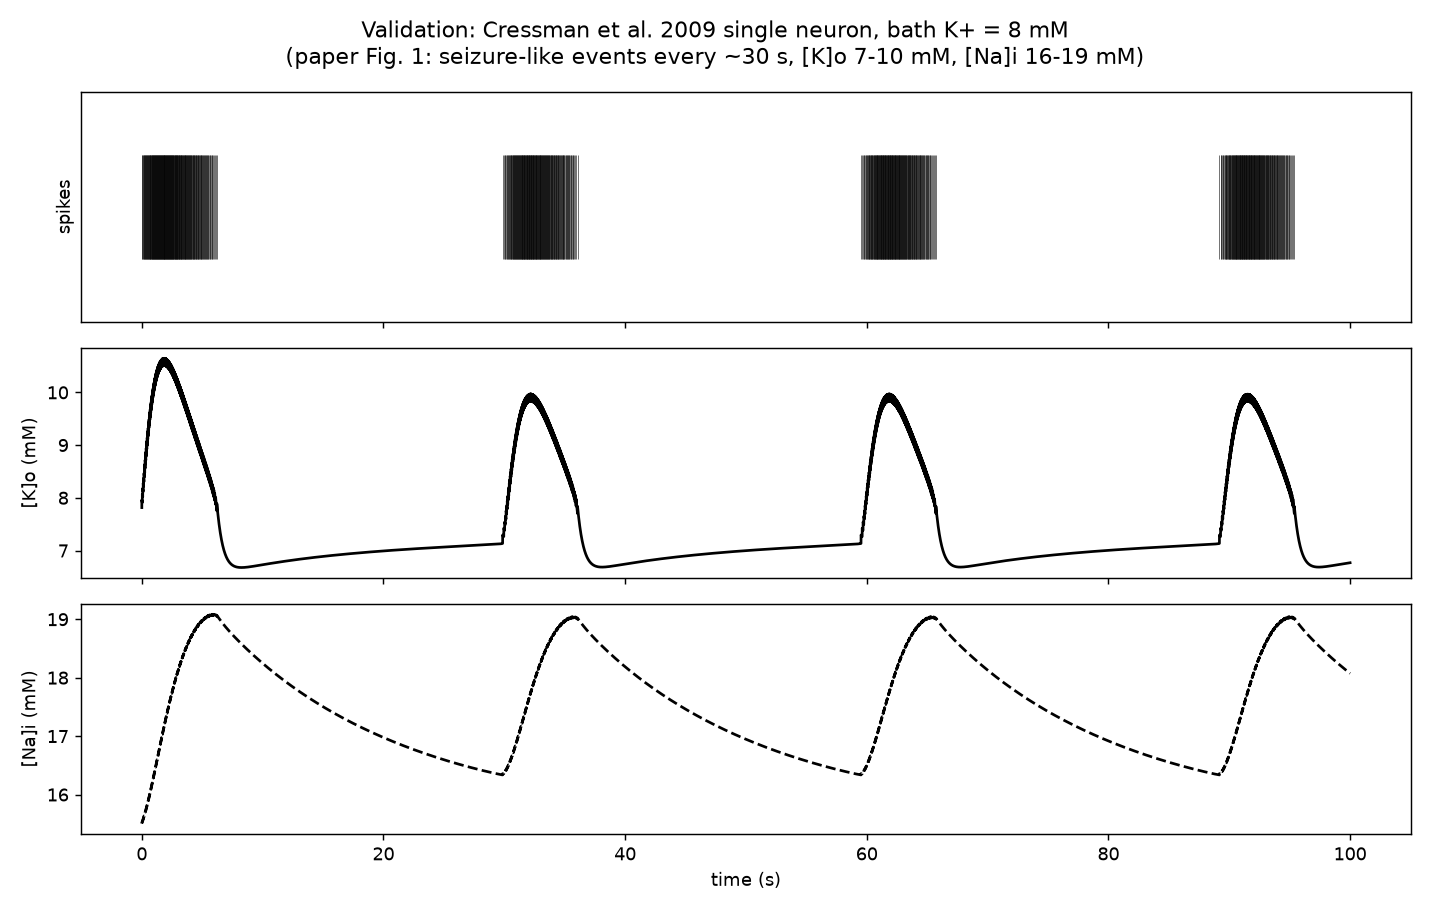
\includegraphics[width=0.7\linewidth]{epilepsy_sim/output/ionic_validation.png}
\caption{Single-neuron validation against Cressman et al.\ 2009, Fig.~1.}
\end{figure}

\subsubsection{Results}

\begin{table}[H]
\centering\small
\caption{Healthy vs epileptic tissue (same neurons, wiring and trigger).}
\label{tab:ionic}
\begin{tabularx}{\linewidth}{@{}l l l L@{}}
\toprule
Measure & Healthy & Epileptic & Real-world reference \\
\midrule
Baseline E firing & 6.1 Hz & 17.3 Hz & Hyperexcitable cortex \\
Resting \Cli{} & 5.6 mM & \best{11.6 mM} & Elevated in human epileptic tissue \\
Resting \EGABA{} (chord) & $-69.6$ mV & \best{$-54.1$ mV} & Depolarised with KCC2 loss \\
Resting \Ko{} & 4.18 mM & 4.59 mM & Impaired buffering \\
Interictal discharges & not epileptiform & \best{33/min} & IEDs on EEG \\
Peak \Ko{} (trigger) & 6.1 mM & \best{12.2 mM} & Ictal \Kp{} ceiling $\approx$10--12 mM \\
Peak \Cli{} & 7.4 mM & \best{15.2 mM} & Ictal \Clm{} loading \\
Peak \EGABA{} & $-63.7$ mV & \best{$-48.3$ mV} & Depolarising GABA \\
Peak \Nai{} & 26.2 mM & 29.8 mM & Ictal \Nap{} loading \\
Peak adenosine & 0.12 & \best{0.68} & Ictal adenosine surge \\
Postictal silence & 13.7 s & \best{25 s} & Postictal depression \\
Minimum \Ko{} after & 3.88 mM & \best{3.66 mM} & Postictal \Kp{} undershoot \\
CBF peak $\to$ minimum & +42\% $\to$ $-47$\% & +31\% $\to$ $-46$\% & Hyperperfusion then hypoperfusion \\
\bottomrule
\end{tabularx}
\end{table}

In epileptic tissue the interictal state shows synchronous population bursts at $\approx$33/min, each sending local \Ko{} to 7--9\,mM with a saw-tooth in \Cli. The trigger drives \Ko{} to the 12\,mM ceiling, \Cli{} to 15.2\,mM (\EGABA{} $-48.3$\,mV, inhibition collapsed), the pump to $\approx$1\,mM/s and adenosine to 0.68 (5.7$\times$ healthy). A 25\,s postictal silence follows with a \Kp{} undershoot to 3.66\,mM (as predicted by Krishnan \& Bazhenov 2011) and CBF falls to $-46$\% (postictal hypoperfusion). The healthy tissue caps \Ko{} near 6\,mM and recovers after a 13.7\,s pump after-hyperpolarisation. The CBF peak is smaller in epileptic tissue because its baseline is already hyperactive.

\begin{figure}[H]
\centering
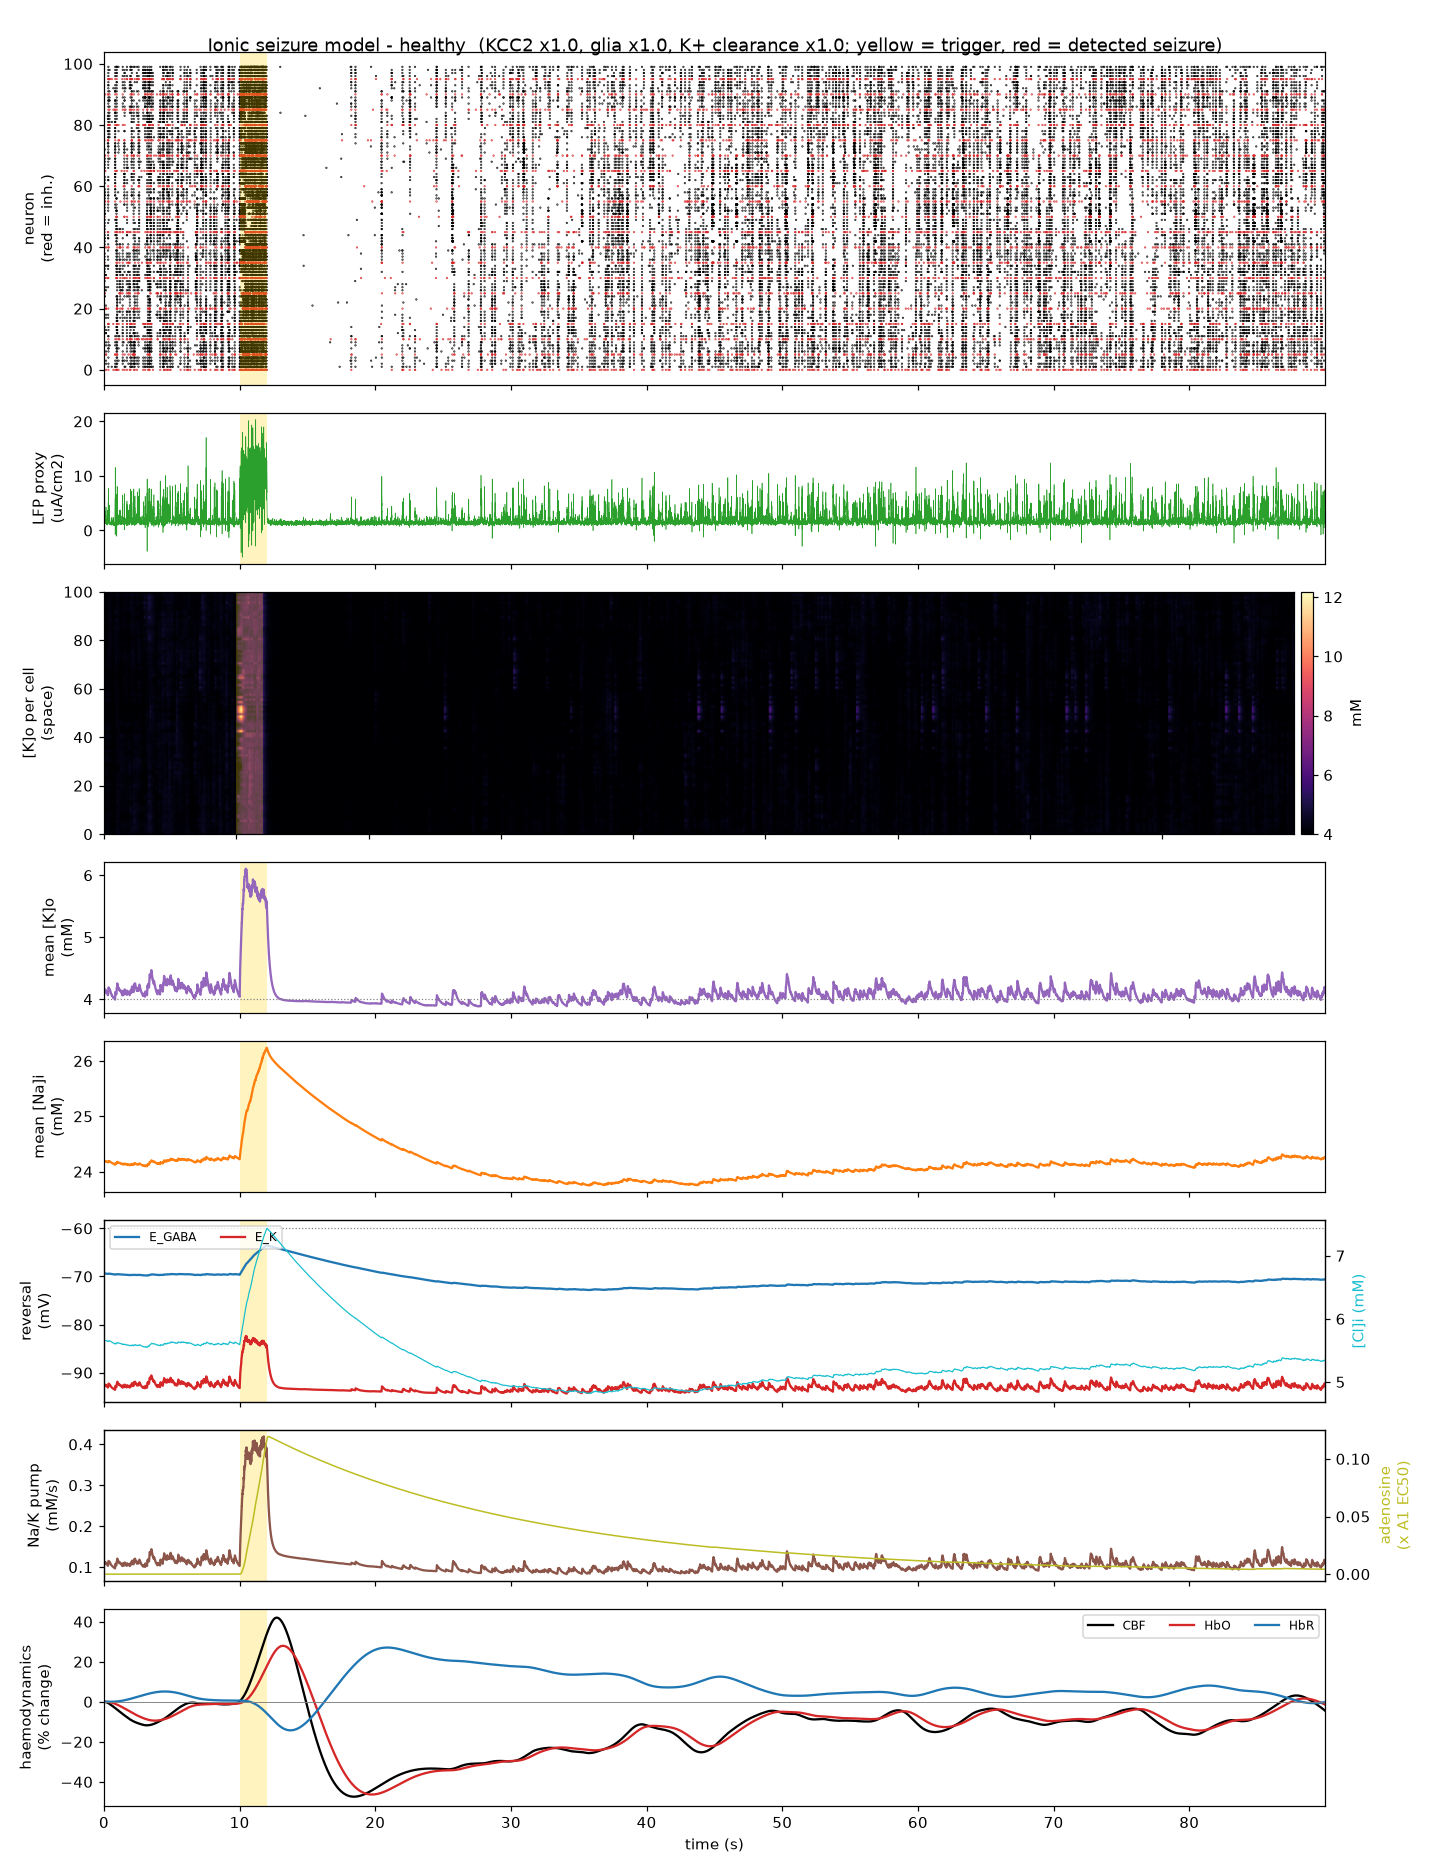
\includegraphics[width=0.49\linewidth]{epilepsy_sim/output/ionic_healthy.png}
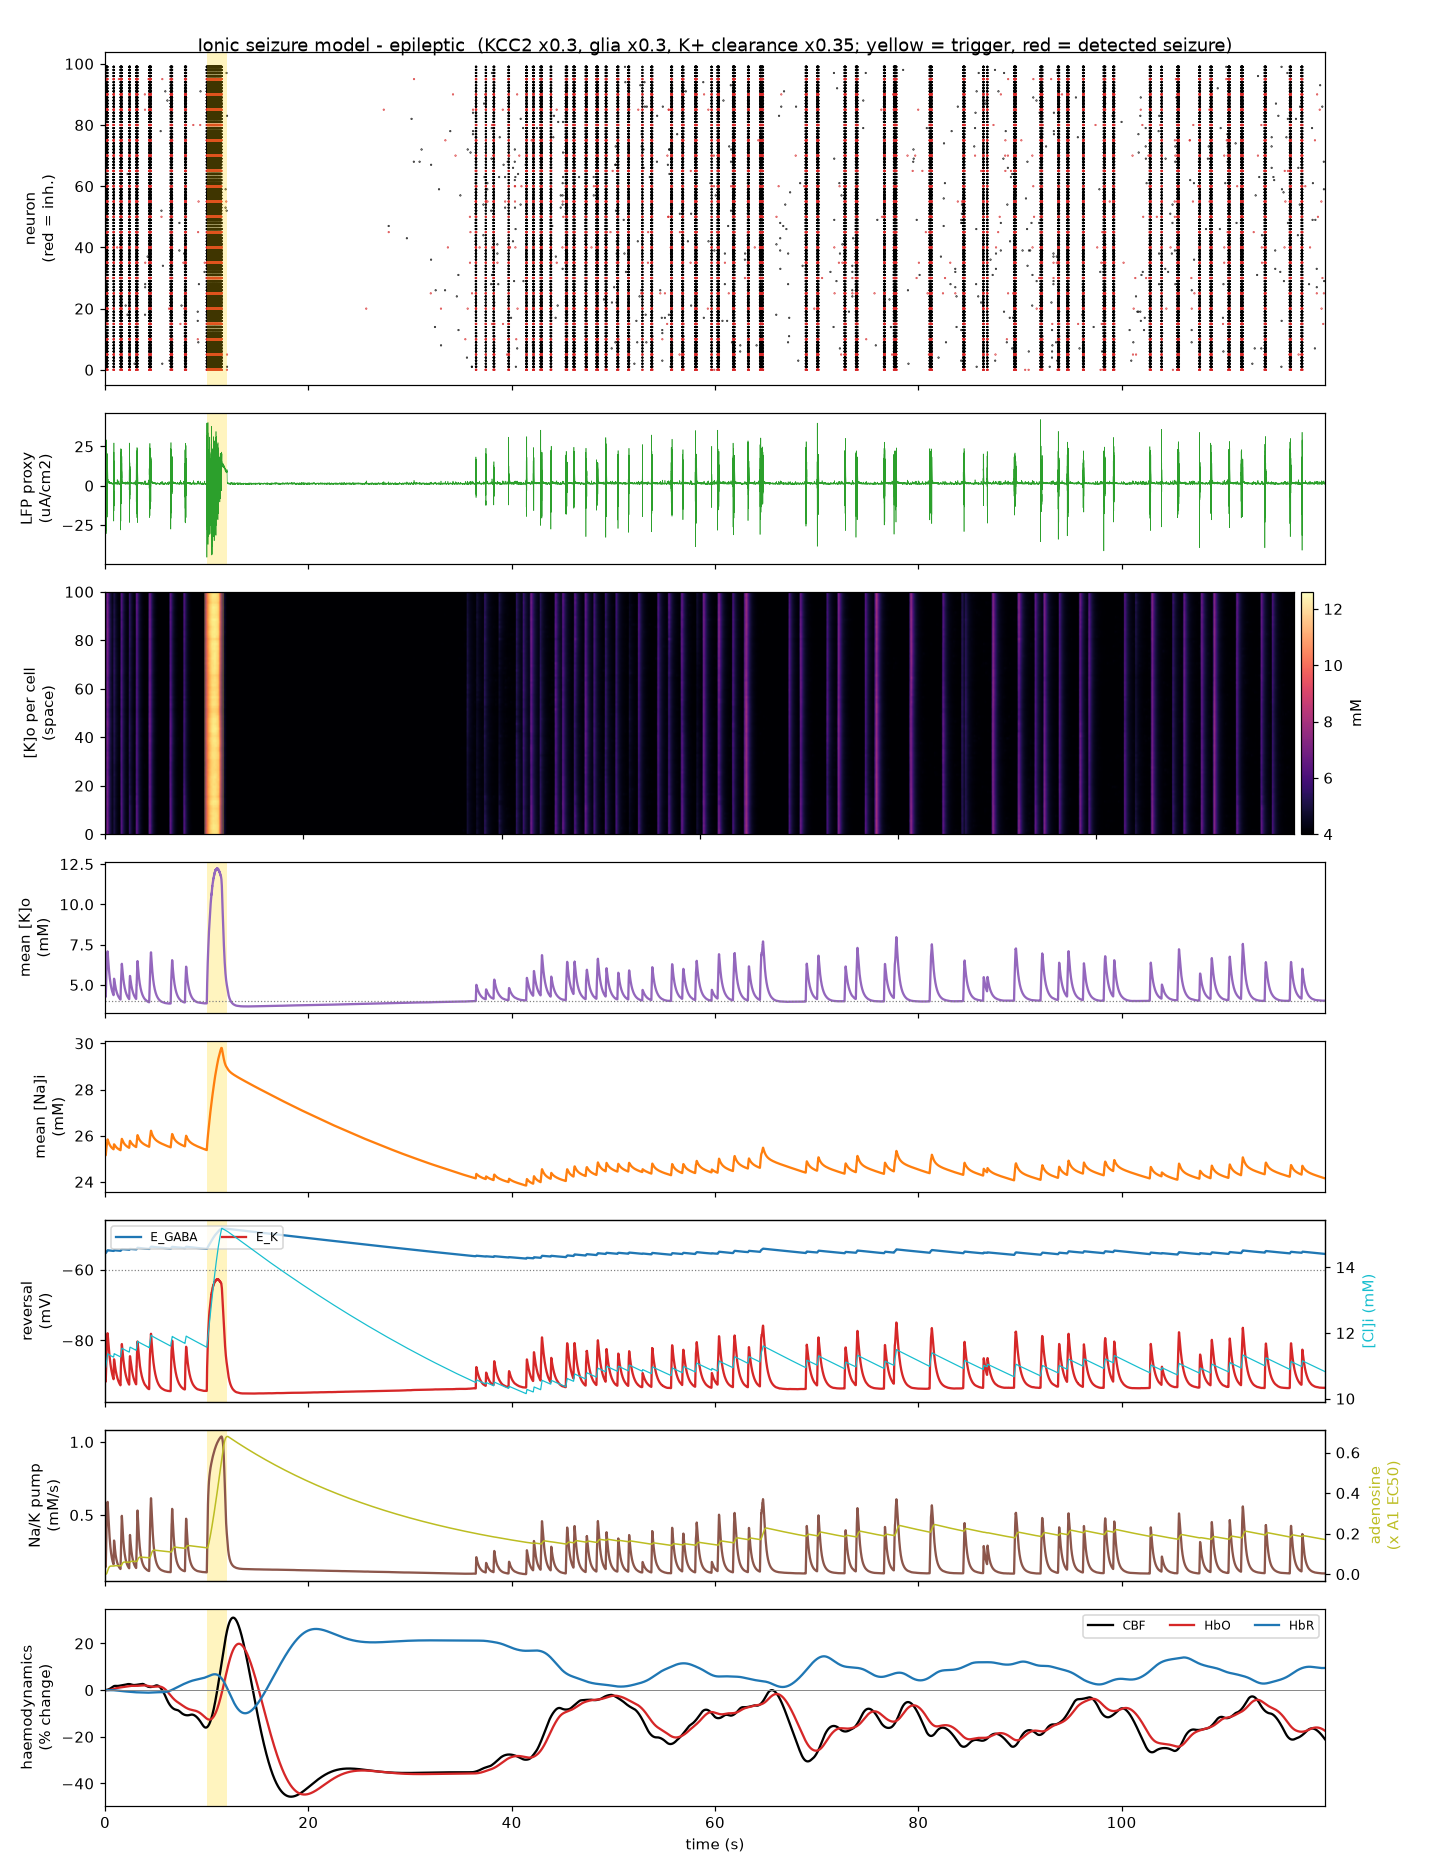
\includegraphics[width=0.49\linewidth]{epilepsy_sim/output/ionic_epileptic.png}
\caption{Ionic model, healthy (left) and epileptic (right): raster, LFP proxy, space--time \Ko{} map, mean \Ko, \Nai, \EGABA/$E_K$/\Cli, pump flux and adenosine, CBF/HbO/HbR.}
\end{figure}

\paragraph{Corrections recorded.} (1) The first E\textsubscript{GABA} values printed ($-70.7$, $-66$, $-57.7$, $-52$\,mV) came from a diagnostic using the GHK form, not the chord form the simulated current obeys; recomputed chord values are $-69.6$, $-63.7$, $-54.1$ and $-48.3$\,mV. The dynamics were unaffected and the code now records the chord form. (2) The healthy ``silence'' metric first printed 0.0\,s because the smoothing window still contained the trigger; the corrected metric searches from 1\,s after the trigger and gives 13.7\,s. (3) The healthy ``36 discharges'' are threshold crossings by normal fluctuations; only rates should be compared.

\subsubsection{Calibration log}

\begin{longtable}{@{}p{0.4cm} p{3.9cm} p{4.6cm} p{5.6cm}@{}}
\caption{Development log: how the ionic model was calibrated.}\\
\toprule
\# & Symptom & Diagnosis & Fix \\
\midrule
\endfirsthead
\toprule
\# & Symptom & Diagnosis & Fix \\
\midrule
\endhead
1 & Printed Cressman equations gave wrong dynamics & Typographical errors in the paper's concentration equations & Used the ModelDB C code ($\gamma=0.0445$, $\div1000$, $\beta$ on $I_K$) per the 2011 erratum \\
2 & -- & Validation & Reproduced Cressman Fig.~1 \\
3 & Baseline firing 245 Hz & One background AMPA event moved $V$ by $\approx$50 mV (tiny leak conductance) & Recalibrated background to 60 Hz $\times$ 0.02 mS/cm\textsuperscript{2} ($\approx$3 Hz) \\
4 & Network locked into permanent 100--200 Hz firing & \Nai{} pinned at 32 mM, no termination & Added electrogenic pump current and \Nap-activated \Kp{} current (Krishnan \& Bazhenov; Compte) \\
5 & E cells silent while I cells fire & Compte's curve assumes resting \Nai{} $\approx$11 mM; here $\approx$19.5 mM & Shifted EC50 38.7$\to$68.6 mM \\
6 & \Nai{} drifting upward & Start state not steady & 60 s warm-up \\
7 & Epileptic tissue did not seize & \Kp{} clearance too fast & Pathology includes glia $\times$0.3 and clearance $\times$0.35 as well as KCC2 loss \\
8 & NaN crash at seizure-level activity & Forward Euler unstable & Exponential Euler (a sign bug in its first version, $v_\infty = v_i + dv/g_{tot}$, was fixed and re-validated) \\
9 & Seizures never terminated & Sustained by depolarising GABA & Tried Tsodyks--Markram depression (U = 0.07, $\tau$ = 700 ms) \\
10 & With depression: no seizures or a 30--50 Hz steady state & Depression caps drive, no slow brake & Depression made optional; adenosine added \\
11 & Per-spike adenosine damped even baseline & Unphysiological & Adenosine proportional to pump ATP use above rest \\
12 & Healthy vs epileptic clearly different & -- & Adopted as default \\
13 & Ictal event stops with the trigger & Pump after-hyperpolarisation 30 mV vs 1--10 mV measured & \code{--pump-i}: at 0.15 seizures self-sustain (10--20 s), self-terminate and recur, but healthy tissue becomes bistable (Gulledge 2013) \\
14 & Sweep at \code{--pump-i 0.35} & Stopped (machine ran low on memory) & Open \\
\bottomrule
\end{longtable}

\subsubsection{Mapping onto real seizure biology, optical readout and limitations}

The model reproduces the ictal \Kp{} ceiling, chloride loading, KCC2 loss, KCC2-mediated \Kp{} loading, interictal discharges, \Nap{} accumulation and pump activation, the adenosine surge, postictal depression, the postictal \Kp{} undershoot, ictal hyperperfusion followed by hypoperfusion, and spatial spread by lateral diffusion; it does \emph{not} yet produce a self-sustained 30--120\,s focal seizure at the default pump setting, and loss of consciousness or motor signs are out of scope. Its bottom panel is what an optical sensor would record: a CBF/HbO surge delayed by seconds during the event and a dip below baseline afterwards; brief interictal events are nearly invisible optically, so optics alone would miss them, while EEG plus optics gives the full picture. Limitations: ictal events are not self-sustaining at default settings; a tiny 1-D network without dendrites, layers, thalamus or long-range connections; one neuron type per population; simplified conservation (no cell swelling); energy implicit (no ATP/O\textsubscript{2}); generic haemodynamics without an initial dip; an LFP proxy rather than a volume-conductor EEG; a simple threshold IED counter; not a clinical tool.
